\chapter{Projekt aplikacji wytwarzania faktur}

\section{Architektura i struktura projektu}
Aplikacja została utworzona za pomocą wzorca projektowego MVVM (Model - View - ViewModel). Wzorzec ten rozwiązuje kilka problemów, z którymi spotykamy się w technologiach Microsoftu:

\begin{itemize}
    \item podział stron/widoków/okien na XAML oraz code-behind
    \item separacja warstw
    \item uproszczenie implementacji złozonych interfejsów
\end{itemize}

Podział wzorca MVVM na model, widok i widok modelu został opisany w książce J. Matulewskiego \cite{MVVMBook} w rozdziałach drugim i trzecim. W drugim rozdziale możemy przeczytać czym tak naprawdę jest rozdzielenie projektu na warstwy modelu, widoku oraz widoku modelu. Z kolei w trzecim autor pisze o implementacji wzroca MVVM. \\
W projekcie został zastosowany dodatkowo wzorzec Dependency Injection (Wstrzykiwanie zależności) z wykorzystaniem IoC (Inversion of Control). Dependency Injection może być zaimplementowane na trzy sposoby:

\begin{enumerate}
    \item Constructor Injection
    \item Setter Injection
    \item Interface Injection
\end{enumerate}

W projekcie zostało zastosowane pierwsze podejście - Constructor Injection, czyli utworzenie instancji obiektu i wstrzyknięcie jej zależności do konstruktora. Dzięki rozwiązaniu Dependency Injection każda instancja wstrzyknięta do konstruktora ma te same dane, co ułatwia nam przesyłanie informacji między obiektami.

\begin{lstlisting}[language={[Sharp]C},label=list:DIinit,caption=Inicjalizacja dependency injection, basicstyle=\footnotesize\ttfamily]
protected override async void OnStartup(StartupEventArgs e)
 {
    InitializeCultures();
    
    var serviceCollection = new ServiceCollection();
    ConfigureServices(serviceCollection);
    ServiceProvider = serviceCollection.BuildServiceProvider();
    ...
    var navigationService = ServiceProvider.GetRequiredService<NavigationService>();
    await navigationService.ShowAsync<MainWindow>();
}
\end{lstlisting}

Na listingu \ref{list:DIinit} został przedstawiony sposób inicjalizacji Dependency Injection w aplikacji. Tworzymy nową instancję klasy ServiceCollection (gdzie będą przechowywane wszystkie zależności). Następnie przekazujemy referencję naszego serviceCollection do funkcji w której zostaną dodane wszystkie zależności, co obserwujemy na listingu \ref{list:DI}

\begin{lstlisting}[language={[Sharp]C},label=list:DI,caption=Konfiguracja dependency injection, basicstyle=\footnotesize\ttfamily]
private void ConfigureServices(IServiceCollection serviceCollection)
{
    serviceCollection.AddDbContext<ApplicationContext>();
    
    serviceCollection.AddScoped<NavigationService>();

    //Services
    serviceCollection.AddScoped(typeof(InvoiceService));
    serviceCollection.AddScoped(typeof(CustomerService));
    serviceCollection.AddScoped(typeof(PaymentTypeService));

    //ViewModels
    serviceCollection.AddTransient(typeof(MainViewModel));
    serviceCollection.AddTransient(typeof(InvoiceViewModel));
    serviceCollection.AddTransient(typeof(InvoiceItemViewModel));
    serviceCollection.AddTransient(typeof(AddCustomerViewModel));

    //Views
    serviceCollection.AddTransient(typeof(MainWindow));
    serviceCollection.AddTransient(typeof(InvoiceWindow));
    serviceCollection.AddTransient(typeof(InvoiceItemWindow));
    serviceCollection.AddTransient(typeof(AddCustomerWindow));
}
\end{lstlisting}

Na początku wstrzyknięta zostaje zależność bazy danych (ApplicationContext) oraz NavigationService (jest potrzebny do poprawnego działania dependency injection oraz uruchamiania widoków. Następnie zostają dodane serwisy, view modele oraz widoki. 
\\\\
Projekt został rozdzielony na dwa osobne podprojekty Core oraz UI. W projekcie Core znajduje się cała logika aplikacji:
\begin{itemize}
    \item Modele,
    \item Serwisy,
    \item View Modele,
    \item Utility - narzędzią, które wspomagają działanie aplikacji
\end{itemize}

\begin{figure}[ht!]
\centering
  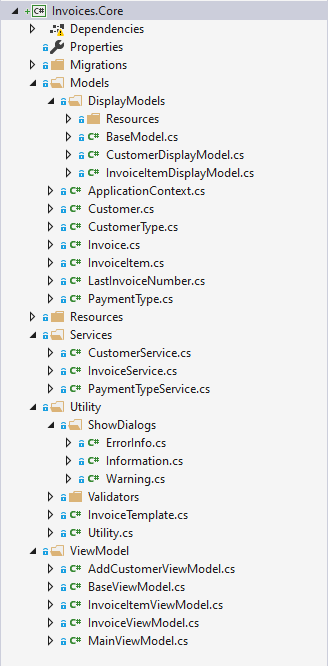
\includegraphics[width=0.5\linewidth]{Rysunki/core.png}
  \caption{Struktura projektu Core}
  \label{fig:Core}
\end{figure}

Z kolei w UI widoki wyświetlane użytkownikowi.

\begin{figure}[ht!]
\centering
  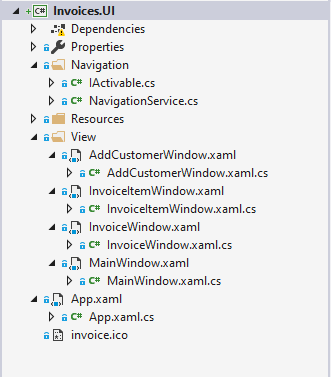
\includegraphics[width=0.5\linewidth]{Rysunki/ui.png}
  \caption{Struktura projektu UI}
  \label{fig:UI}
\end{figure}

\section{Podstawowe obiekty aplikacji\label{AppObjects}}
Rysunek \ref{fig:classDiagram} przedstawia klasy znajdujące się w aplikacji. Wyróżniamy 3 główne klasy oraz 3 pomocnicze (w przyszłości mogą zostać rozbudowane). 

\begin{figure}[ht!]
  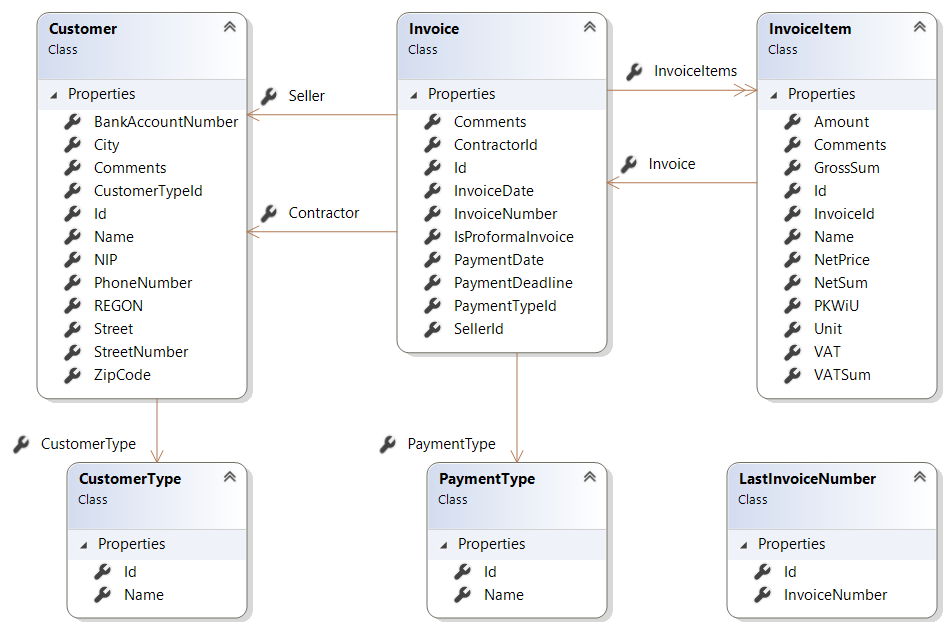
\includegraphics[width=\linewidth]{Rysunki/ClassDiagram.png}
  \caption{Diagram klas}
  \label{fig:classDiagram}
\end{figure}

\subsection{Customer}
Klasa Customer reprezentuje klienta aplikacji. Rozróżniamy dwa typy klientów: Kontrahent (osoba dla której wystawiamy fakturę) oraz Sprzedawca (osoba wystawiająca fakturę).
\\\\
Właściwości:
\begin{itemize}
    \item Name - imię i nazwisko klienta/firmy
    \item City - miasto, w którym klient urzęduje lub w którym znajduje się firma
    \item ZipCode - kod pocztowy
    \item Street - ulica, na której klient mieszka lub na której znajduje się firma
    \item StreetNumber - numer domu i mieszkania
    \item PhoneNumber - numer telefonu klienta/firmy
    \item NIP - Numer identyfikacji podatkowej
    \item REGON - (Rejestr Gospodarki Narodowej), Krajowy Rejestr Urzędowy Podmiotów Gospodarki Narodowej
    \item BankAccountNumber - numer konta bankowego klienta/firmy
    \item Comments - uwagi do klienta/firmy
    \item CustomerType - jest to instancja klasy CustomerType, która definiuje role klienta (Kontrahent, Sprzedawca)
    \item CustomerTypeId - pomocnicza zmienna pozwalająca w łatwy sposób odczytać typ klienta.
\end{itemize}

\subsection{Invoice}
Klasa Invoice reprezntuje faktury w aplikacji. Jest to najważniejsza klasa w całej aplikacji.
\\\\
Właściwości:
\begin{itemize}
    \item InvoiceNumber - numer faktury, ustalany na podstawie poprzedniego numeru faktury (format: kolejny numer/rok).
    \item InvoiceDate - data wysatwienia faktury
    \item PaymentDeadline - ostateczny termin płatności za fakturę
    \item PaymentDate - data kiedy faktura została opłacona
    \item IsProformaInvoice - czy faktura jest fakturą pro forma
    \item Comments - uwagi do faktury
    \item Contractor - jest to instancja klasy Customer, która definiuje kto jest kontrahentem na fakturze
    \item Seller - jest to instancja klasy Customer, która definiuje kto jest sprzedawcą na fakturze
    \item PaymentType - jest to instancja klasy PaymentType, która definiuje metodę płatności za fakturę
    \item InvoiceItems - jest to kolekcja przedmiotów/produktów, które znajdują się na fakturze
    \item ContractorId oraz SellerId - dwie pomocnicze zmienne pozwalające w łatwy sposób odczytać klienta.
    \item PaymentTypeId - pomocnicza zmienna pozwalająca w łatwy sposób odczytać rodzaj płatności.
\end{itemize}

\subsection{InvoiceItem}
Klasa InvoiceItem reprezentuje przedmioty, które znajdują się na fakturze. Bez produktow faktura nie może zostać utworzona.
\\\\
Właściwości:
\begin{itemize}
    \item Name - nazwa produktu
    \item PKWiU - Polska Klasyfikacja Wyrobów i Usług
    \item Unit - jednostka w jakiej jest kupowany przedmiot (sztuki, opakowania, kilogramy)
    \item NetPrice - cena netto produktu
    \item Amount - ilość kupowanego produktu
    \item NetSum - suma netto kupowanego produktu, jest to cena netto pomnożona razy ilość kupowanego produktu
    \item VAT - podatek VAT podawany w procentach
    \item GrossSum - suma brutto kupowanego produktu, jest to suma netto pomnożona razy podatek VAT
    \item VATSum - suma podatku VAT, jest to różnica sumy brutto i sumy netto produktu
    \item Comments - uwagi do produktu
    \item Invoice - jest to instancja klasy Invoice, która ma na celu zidentyfikowanie do jakiej faktury należy dany produkt
    \item InvoiceId - pomocniczna zmienna pozwalająca odczytać fakturę
\end{itemize}

\subsection{CustomerType}
CustomerType to pomocnicza klasa pozwalająca zidentyfikować rodzaj klienta. Klasa ta posiada jedną właściwość jaką jest nazwa klienta (Kontrahent, Sprzedawca).

\subsection{PaymentType}
PaymentType to pomocnicza klasa pozwalająca zidentyfikować rodzaj płatności. Klasa ta posiada jedną właściwość jaką jest nazwa płatności (Gotówka, Przelew lub płatność kartą).

\subsection{LastInvoiceNumber}
LastInvoiceNumber to pomocnicza klasa pozwalająca na wygenerowanie nowego numeru porządkowego faktury. Posiada jedną właściwość jaką jest numer faktury (jest to ostatni numer faktury z danego roku). 

\section{Implementacja aplikacji} %Projekt przypadków użycia
Na poniższych rysunkach zostały przedstawione zależności pomiędzy pozostałymi klasami, widokami oraz modelami widoków w projekcie, a także metody, które znajdują się w poszczególnych klasach.

W aplikacji zostały utworzone dwie dodatkowe klasy DisplayModels, które ułatwiają wyświetlanie oraz wprowadzanie danych przez użytkownika. Obie te klasy dziedziczą po abstrakcyjnej klasie BaseModel. Klasa BaseModel implementuje 2 główne funkcje:

\begin{itemize}
    \item SetProperty<T> - metoda informuje widok, że nastąpiła zmiana w którejś z właściwości (użytkownik wprowadził zmianę)
    \item ValidateProperty<T> - metoda służy do sprawdzenia poprawności wpisanych danych przez użytkownika
\end{itemize}

Na rysunku \ref{fig:displayModelsDiagram} zostały przedstawione klasy CustomerDisplayModel i InvoiceItemDisplayModel, które posiadają takie same pola co klasy im odpowiadające (Customer oraz InvoiceItem). Jedyną różnicą jest to, że w klasach DisplayModels wszystkie pola są typu string.

\begin{figure}[ht!]
  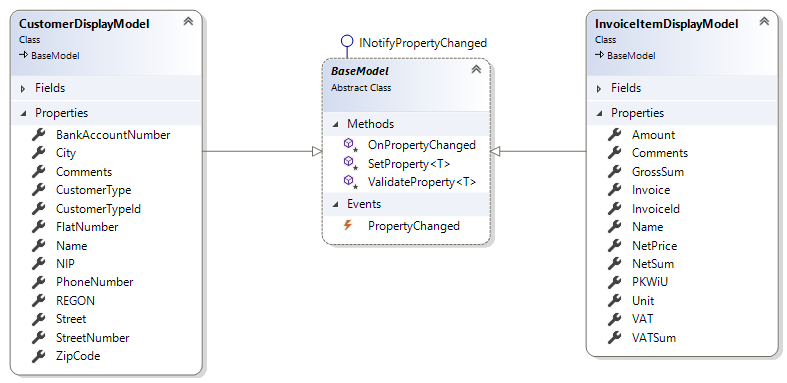
\includegraphics[width=\linewidth]{Rysunki/DisplayModelsDiagram.png}
  \caption{Diagram pomocniczych modeli}
  \label{fig:displayModelsDiagram}
\end{figure}

\subsection{AddCustomer}

\subsubsection{ViewModel}
Na rysunku \ref{fig:addCustomerViewModelDiagram} przedstawiony został, wraz ze związkami z innymi klasami, diagram viewmodelu dodawania klienta. 

\begin{figure}[ht!]
  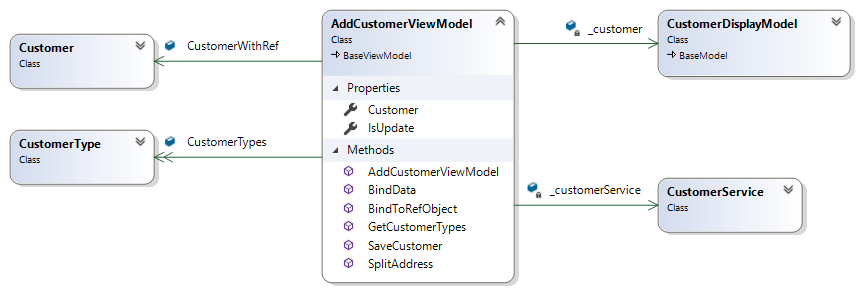
\includegraphics[width=\linewidth]{Rysunki/AddCustomerViewModelDiagram.png}
  \caption{Diagram modelu widoku dodawania klienta}
  \label{fig:addCustomerViewModelDiagram}
\end{figure}

Właściwość CustomerWithRef jest referencją przekazanego do view modelu obiektu, przez co później łatwiej edytować obiekty.
Atrybuty pola \_customer są związane z poszczególnymi kontrolkami na widoku AddCustomerWindow. Przez taki zabieg nie musimy się martwić o sczytywanie zawartości, ponieważ mamy je odrazu w atrybutach obiektu \_customer. 
\\
W konstruktorze wstrzykiwana jest zależność \_customerService, przez co nie musimy się martwić przekazywaniem obiektu typu CustomerService, gdy tworzymy nową instancję AddCustomerViewModel. Metody BindData oraz BindToRefObject służą przygotowaniu wprowadzonych danych do zapisania. Metoda SplitAddress, dzieli otrzymany numer budynku oraz lokalu (są połączone) na dwie osobne wartości. 

Ważniejsze metody:

\begin{enumerate}
    \item \textbf{BindData} \\
    Metoda służy przypisaniu przychodzących danych do obiektu wyświetlanego na widoku. Przed każdym przypisaniem sprawdzane jest czy dana nie jest pusta. 
    \\
    \item \textbf{BindDataToRef} \\
    Metoda przypisuje obiekt wyświetlany na widoku do obiektu przekazanego poprzez referencję. 
    \\
    \item \textbf{SplitAddress} \\
    Metoda rozdziela numer na dwa osobne obiekty (numer budynku oraz numer lokalu). W bazie danych te dwa numery trzymane są jako jeden obiekt
\end{enumerate}

\subsubsection{View}
Klasa AddCustomerWindow (rysunek \ref{fig:addCustomerWindowDiagram}) implementuje interfejs IActivable, dzięki któremu jesteśmy w stanie przekazywać parametry do widoku. Posiada również pole ViewModel typu AddCustomerViewModel (konwencja MVVM).

\begin{figure}[ht!]
\centering
  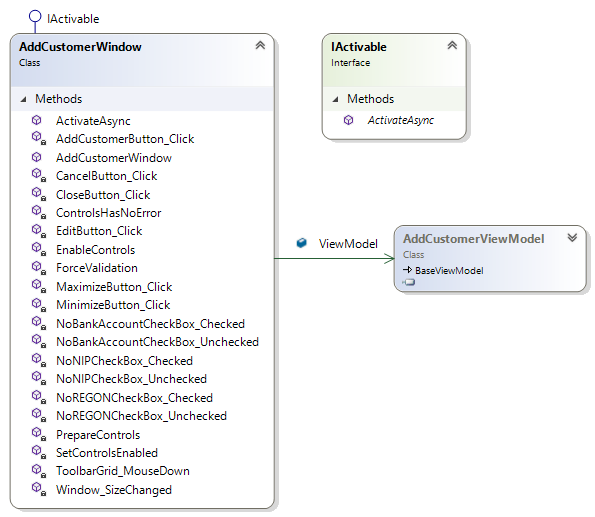
\includegraphics[width=0.7\linewidth]{Rysunki/AddCustomerWindowDiagram.png}
  \caption{Diagram klasy widoku dodawania klienta}
  \label{fig:addCustomerWindowDiagram}
\end{figure}

Ważniejsze metody:

\begin{enumerate}
    \item \textbf{ActivateAsync} \\
    Metoda jest zaimplementowana z interfejsu \textbf{IActivable} i wywoływana przed pokazaniem widoku. Funkcja przyjmuje parametr, dzięki czemu jesteśmy w stanie przekazać dowolny obiekt do naszego widoku. W metodzie zostaje przygotowany obiekt (przypisanie danych do obiektu, wypełnienie kontrolek odpowiednimi danymi), który zostanie wyświetlony w oknie, dlatego ważnym jest, żeby metoda uruchomiła się przed załadowaniem widoku. 
    \\
    \item \textbf{AddCustomerButton\_Click} \\
    Jest to jedna z ważniejszych metod w widoku. Wywoływana jest kliknięciem w przycisk i zapisuje obiekt Customer w bazie danych. Funkcja sprawdza na początku czy wszystkie dane zostały wprowadzone prawidłowo (jeżeli nie, dostajemy stosowny komunikat). Następnie wszystkie dane zostają przypisane do obiektu z referencją i obiekt zapisywany jest w bazie danych.
    \\
    \item \textbf{ForceValidation} \\
    Metoda niejawnie aktualizuje kontrolki. Po takim zabiegu jeżeli jakaś kontrolka nie została uzupełniona lub została uzupełniona błędnie otrzymamy stosowny komunikat (nie będziemy też w stanie zapisać obiektu Customer).
\end{enumerate}


\subsubsection{Service}
CustomerService odpowiada za połączenie z bazą danych a także operacje CRUD (Create, Read, Update, Delete). Na listingu \ref{list:CustomerSUD} zostały przedstawione metody do zapisu, zaktualizowania oraz usunięcia obiektu Customer.

\begin{lstlisting}[language={[Sharp]C},label=list:CustomerSUD,caption=Przykładowe metody w serwisie CustomerService, basicstyle=\footnotesize\ttfamily]
public void SaveCustomer(Customer customerWithRef)
{
    _ctx.Customers.Add(customerWithRef);
    _ctx.SaveChanges();
}

public void UpdateCustomer(Customer customerWithRef)
{
    var oldCustomer = _ctx.Customers.Find(customerWithRef.Id);

    _ctx.Entry(oldCustomer).CurrentValues.SetValues(customerWithRef);
    _ctx.SaveChanges();
}

public void DeleteCustomer(Customer customer)
{
    _ctx.Customers.Remove(customer);
    _ctx.SaveChanges();
}
\end{lstlisting}

Wszystkie zapytania do bazy realizowane są za pomocą Entity Framework Core. 

\subsection{Invoice}

\subsubsection{ViewModel}
Na rysunku \ref{fig:InvoiceViewModelDiagram} przedstawiony został diagram klasy InvoiceViewModel. 

\begin{figure}[ht!]
  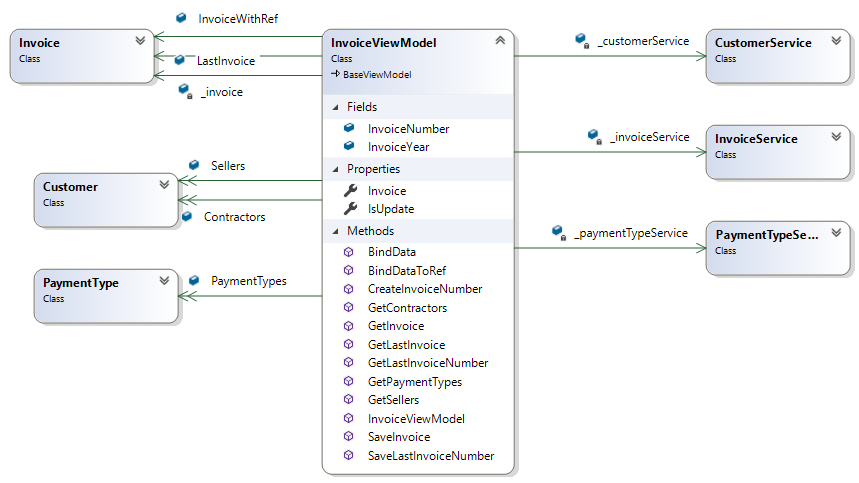
\includegraphics[width=\linewidth]{Rysunki/InvoiceViewModelDiagram.png}
  \caption{Diagram modelu widoku faktur}
  \label{fig:InvoiceViewModelDiagram}
\end{figure}

Obiekt InvoiceWithRef trzyma referencję do oryginalnego obiektu faktury (potrzebne przy aktualizacji faktur). LastInvoice jest ostatnią fakturą dodaną do bazy danych. Jest potrzebna w celu ustalenia kolejnego numeru porządkowego faktury. Właściwość Invoice została utworzona w celu wyświetlenia oraz późniejszego sczytania wartości z widoku. Do InvoiceViewModel zostają wstrzyknięte 3 serwisy które dostarczają oraz pozwalają zapisać nasze dane w bazie. Klasa InvoiceViewModel posiada także dwa obiekty typu Customer, które identyfikują kontrahenta oraz sprzedawcę. Model widoku posiada również 3 kolekcje, które oznaczone są na diagramie przez podwóją strzałkę. Listy dostarczają nam wszystkich kontrahentów oraz sprzedawców, a także typy płatności za faktury.

Ważniejsze metody:
\begin{enumerate}
    \item \textbf{BindData oraz BindDataToRef} - metody bardzo podobne do opisanych wcześniej (przy AddCustomer), służą do przypisania przychodzących oraz wychodzących danych.
    \item \textbf{CreateInvoiceNumber} \\
    Metoda generuje kolejny numer porządkowy (na podstawie ostatniej faktury) przy tworzeniu nowej faktury. Jako parametr metody jest przekazywany ostatni numer porządkowy. W przypadku, gdy rok jest ten sam liczba zwiększa się o jeden, gdy rozpoczyna się nowy rok, numeracja startuje od początku i rok jest aktualizowany.
\end{enumerate}

\subsubsection{View}
Na rysunku \ref{fig:InvoiceWindowDiagram} został przedstawiony diagram klasy widoku faktur. Klasa implementuje interfejs IActivable. Interfejs ten dostarcza nam metodę \textbf{ActivateAsync}, która przyjmuje parametr, dzięki czemu jesteśmy w stanie przekazać obiekt do naszego widoku.

\begin{figure}[ht!]
\centering
  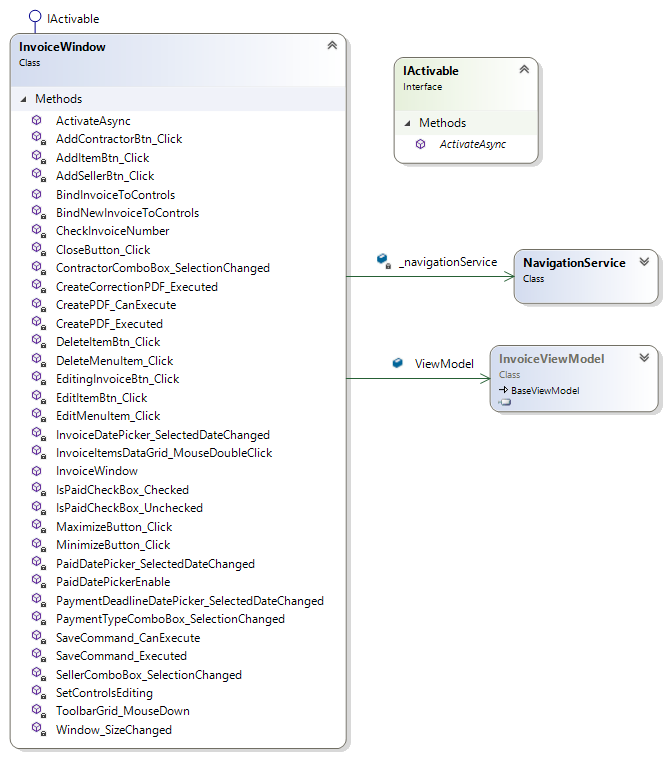
\includegraphics[width=0.7\linewidth]{Rysunki/InvoiceWindowDiagram.png}
  \caption{Diagram widoku faktur}
  \label{fig:InvoiceWindowDiagram}
\end{figure}

Klasa posiada dwa obiekty. Pierwszy z nich to InvoiceViewModel, w którym jest zaimplementowana cała logika. Drugi to NavigationService, który pozwala uruchomić kolejne okna z zachowaniem dependency injection. 

Ważniejsze metody:
\begin{enumerate}
    \item \textbf{AddContractorBtn\_Click} i \textbf{AddSellerBtn\_Click} \\
    Metoda uruchamia widok, w którym możemy dodać nowego kontrahenta, bądź sprzedawcę. Funkcja korzysta z zależności NavigationService w celu poprawnego uruchomienia okna. Przed dodaniem sprawdzane jest czy obiekt nie jest pusty.
    \item \textbf{AddItemBtn\_Click} \\
    Funckja pozwala na dodanie nowej pozycji na fakturze. Zostaje uruchomione nowe okno (InvoiceItemWindow), w którym dodajemy pozycję na fakturę.
    \item \textbf{BindInvoiceToControls} \\
    Metoda przypisuje odpowiednie właściwości obiektu Invoice to kontrolek, które wyświetlane są na widoku. Funkcja jest uruchamiana w trakcie edycji faktury i ma swój odpowiednik w przypadku tworzenia nowej faktury.
    \item \textbf{BindNewInvoiceToControls} \\
    Funkcja działa tak jak wyżej tylko uruchamiana jest przy tworzeniu nowej faktury.
    \item \textbf{CheckInvoiceNumber} \\
    Metoda sprawdza poprawność utworzonego numeru porządkowego faktury. Tworzy też nowy numer porządkowy w przypadku ustawienia daty wystawienia faktury na kolejny rok.
    \item \textbf{CreatePDF\_Executed} i \textbf{CreateCorrectionPDF\_Executed} \\
    Metody tworzą kolejno plik PDF z wybraną przez użytkownika fakturą oraz korektę do faktury (jeżeli na fakturze pojawiły się jakieś zmiany). 
    \item \textbf{DeleteItemBtn\_Click} i \textbf{DeleteMenuItem\_Click} \\
    Obie metody pozwalają na usunięcie pozycji z faktury, w przypadku niezaznaczenia produktu, aplikacja wyświetla stosowny komunikat. 
    \item \textbf{EditItemBtn\_Click}, \textbf{EditMenuItem\_Click} oraz \\
    \textbf{InvoiceItemsDataGrid\_MouseDoubleClick} \\
    Obie metody pozwalają na edytowanie pozycji z faktury, w przypadku niezaznaczenia produktu, aplikacja wyświetla stosowny komunikat. 
    \item \textbf{SaveCommand\_Executed} \\
    Metoda na początku sprawdza czy kontrahent oraz sprzedawca zostali wybrani prawidłowo (oraz czy w ogóle zostali wybrani). Następnie przypisuje wszystkie właściwości do obiektu z referencją i zapisuje fakturę w bazie.
\end{enumerate}

Metody z dopiskiem \textbf{\_SelectedDateChanged} sprawdzają czy wszystkie daty na fakturze zostały wprowadzone prawidłowo. W przypadku podania złych dat aplikacja wyświetla odpowiedni komunikat. 

\subsubsection{Service}
Na listingu \ref{list:InvoiceService} zostały przedstawione przykładowe metody operacji CRUD. 

\begin{lstlisting}[language={[Sharp]C},label=list:InvoiceService,caption=Przykładowe metody w serwisie InvoiceService, basicstyle=\footnotesize\ttfamily]
public List<Invoice> GetInvoices()
{
    return _ctx.Invoices
        .Include(p => p.InvoiceItems)
        .Include(seller => seller.Seller)
        .Include(contractor => contractor.Contractor)
        .Include(paymentType => paymentType.PaymentType)
        .ToList();
}

public Invoice GetInvoice(int id)
{
    return _ctx.Invoices
        .Include(x => x.PaymentType)
        .Include(x => x.InvoiceItems)
        .Include(x => x.Contractor)
        .Include(x => x.Seller)
        .FirstOrDefault(x => x.Id == id);
}

public void DeleteInvoice(Invoice invoice)
{
    _ctx.Invoices.Remove(invoice);
    _ctx.SaveChanges();
}

public void SaveInvoice(Invoice invoice)
{
    _ctx.Invoices.Add(invoice);
    _ctx.SaveChanges();
}

public void UpdateInvoice(Invoice invoice)
{
    var oldInvoice = _ctx.Invoices.Find(invoice.Id);

    _ctx.Entry(oldInvoice).CurrentValues.SetValues(invoice);
    _ctx.SaveChanges();
}
\end{lstlisting}

Pierwsza z metod \textbf{GetInvoices} pobiera z bazy danych listę wszystkich faktur i dołącza do nich odpowiadające im obiekty InvoiceItems, Customer oraz PaymentType za pomocą funkcji \textbf{Include} dostarczanej przez Entity Framework Core. 

\subsection{InvoiceItem}
\subsubsection{ViewModel}
Na rysunku \ref{fig:InvoiceItemDiagram} został przedstawiony diagram klasy InvoiceItemViewModel. Klasa ta posiada 2 główne obiekty (podobnie jak pozostałem klasy ViewModel):

\begin{enumerate}
    \item InvoiceItem (typu InvoiceItemDisplayModel) - obiekt wyświetlany oraz bindowany do widoku
    \item InvoiceItemWithRef (typu InvoiceItem) - obiekt z referencją, zapisywany do bazy danych
\end{enumerate}

\begin{figure}[ht!]
  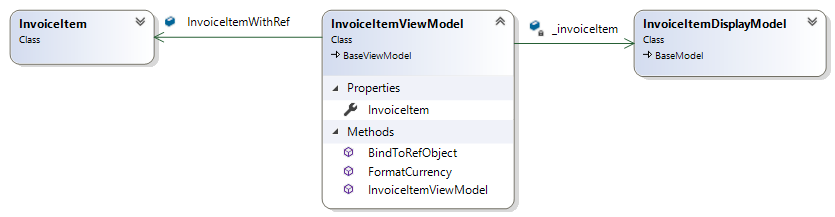
\includegraphics[width=\linewidth]{Rysunki/InvoiceItemViewModelDiagram.png}
  \caption{Diagram modelu widoku InvoiceItem}
  \label{fig:InvoiceItemDiagram}
\end{figure}

InvoiceItemViewModel posiada dwie ważne metody:

\begin{enumerate}
    \item \textbf{BindToRefObject} \\
    Tak jak w pozostałych modelach widoku, w metodzie zostają przypisane wartości, wprowadzone przez użytkownika, z obiektu InvoiceItem do obiektu z referencją InvoiceItemWithRef. 
    \item \textbf{FormatCurrency} \\
    Metoda została utworzona w celu poprawnej konwersji waluty na format polski.
\end{enumerate}

\subsubsection{View}
Na rysunku \ref{fig:InvoiceItemWindowDiagram} został przedstawiony diagram klasy widoku pozycji z faktury. Klasa implementuje interfejs IActivable. 

\begin{figure}[ht!]
\centering
  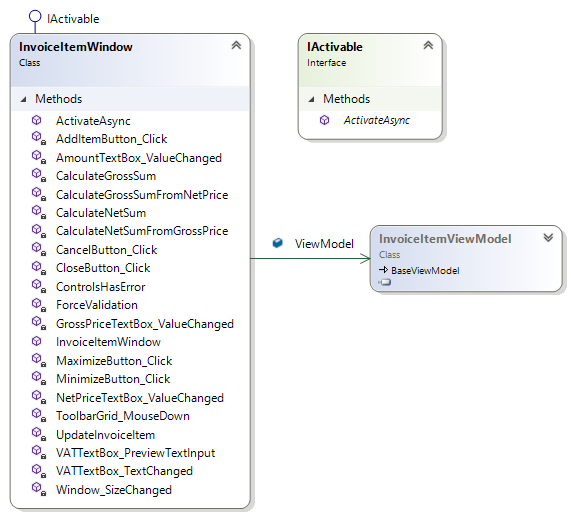
\includegraphics[width=0.7\linewidth]{Rysunki/InvoiceItemWindowDiagram.png}
  \caption{Diagram widoku modelu InvoiceItem}
  \label{fig:InvoiceItemWindowDiagram}
\end{figure}

Klasa posiada jeden główny obiekt InvoiceItemViewModel, który implementuje cała logikę widoku.
\\
Ważniejsze metody:
\begin{enumerate}
    \item \textbf{ActivateAsync} \\
    Metoda została zaimplementowana z interfejsu \textbf{IActivable}. Funkcja pozwala nam na przekazanie dowolnego obiektu do naszego widoku. Następnie w metodzie obiekt zostaje przygotowany i podpięty do kontrolek, by później móc zostać poprawnie wyświetlony. 
    \item \textbf{AddItemButton\_Click}\\
    Jest to najważniejsza metoda w widoku. Wywoływana jest poprzez kliknięcie przycisku zapisywania pozycji. Funkcja sprawdza na początku czy wszystkie dane zostały wpisane prawidłowo. Jeżeli dane zostały wprowadzone źle aplikacja informuje nas komunikatem, w przeciwnym razie pozycja zostaje dodana do faktury.
    \item \textbf{ForceValidation} i \textbf{ControlsHasNoError} \\
    Obie metody służą do walidacji wpisanych przez użytkownika danych. Pierwsza z nich niejawnie aktualizuje kontrolkę w celu wywołania walidacji, z kolei druga sprawdza czy, na którejś kontrolce, wystąpił błąd walidacji.
\end{enumerate}

Funkcje z dopiskiem \textbf{\_ValueChanged} oraz \textbf{\_TextChanged} na bieżąco obliczają wartości: 
\begin{itemize}
    \item Ceny netto
    \item Ceny brutto
    \item Sumy netto
    \item Sumy brutto
    \item Sumy VAT
\end{itemize}

\subsubsection{Service}
W przypadku InvoiceItem serwis nie został utworzony, ponieważ nie było takiej potrzeby. Wszystkie zapytania związane z dodawaniem, usuwaniem i czytaniem pozycji z faktury realizowane są automatycznie przy dodawaniu nowego/edycji obiektu Invoice.

\subsection{Main}

\subsubsection{ViewModel}
Rysunek \ref{fig:MainViewModelDiagram} przedstawia diagram widoku modelu MainViewModel. ViewModel posiada 3 główne kolekcje, które dostarczają dane do naszego widoku. Do MainViewModel zostały wstrzyknięte 2 serwisy: InvoiceService (pobiera dane faktur z bazy) i CustomerService (pobiera dane kontrahentów oraz sprzedawców z bazy). Widok modelu nie posiada skomplikowanych funkcji, ponieważ został stworzony tylko do wyświetlania oraz usuwania danych. \\
Ważniejszą metodą jest \textbf{DeleteInvoice}. Funkcja nie tylko usuwa wybraną przez użytkownika fakturę, ale także zmienia koljeny numer porządkowy faktury. Numeracja faktur musi odbywać się po kolei i powinna być ciągła.

\begin{figure}[ht!]
  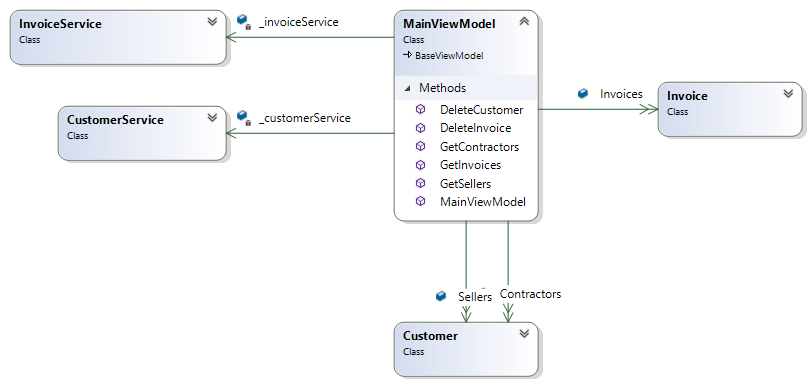
\includegraphics[width=\linewidth]{Rysunki/MainViewModelDiagram.png}
  \caption{Diagram głównego modelu widoku}
  \label{fig:MainViewModelDiagram}
\end{figure}

\subsubsection{View}
Na rysunku \ref{fig:MainWindowDiagram} został przedstawiony diagram głównego widoku aplikacji. MainWindow ma wstrzyknięte 2 zależności: NavigationService (służący do otwierania koljenych widoków) i MainViewModel (widok modelu). 
\\
Ważniejsze metody:
\begin{enumerate}
    \item \textbf{AddContractorButton\_Click} i \textbf{AddSellerButton\_Click} \\
    Metoda otwiera asynchroniczny widok (AddCustomer), który umożliwia dodanie nowego sprzedawcy lub kontrahenta, w zależności od wybranego typu.
    \item \textbf{AddInvoiceButton\_Click} \\
    Funkcja otwiera asynchroniczny widok (Invoice), pozwalający na dodanie nowej faktury.
    \item \textbf{SearchInvoiceTextBox\_KeyUp} \\
    Metoda służy do wyszukiwania faktur. Faktury można wyszukać po: numerze faktury, nazwie (kontrahenta, sprzedawcy), ulicy i mieście (kontrahenta) oraz dacie wystawienia.
    \item \textbf{SearchSellerTextBox\_KeyUp} i \textbf{SearchContractorTextBox\_KeyUp} \\
    Metody służą do wyszukania sprzedawcy/kontrahenta. Osoby te możemy wyszukać po: nazwie, NIPie, REGONie, ulicy oraz mieście.
\end{enumerate}

Metody z dopiskiem \textbf{\_MouseDoubleClick} służą do edytowania faktury, kontrahenta i sprzedawcy. Funkcja wywyołuje się podczas dwukkrotnego kliknięcia w pozycję na liście.

\begin{figure}[ht!]
\centering
  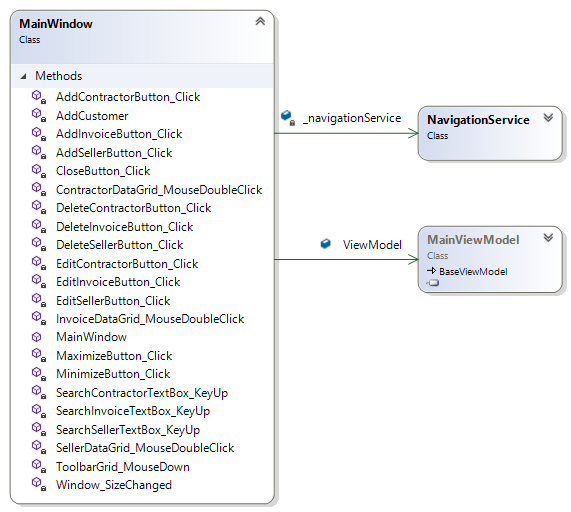
\includegraphics[width=0.7\linewidth]{Rysunki/MainWindowDiagram.png}
  \caption{Diagram głównego widoku}
  \label{fig:MainWindowDiagram}
\end{figure}

\subsubsection{Service}

W przypadku Main serwis nie został utworzony. Widok główny korzysta z serwisów \textbf{InvoiceService} oraz \textbf{CustomerService}, które dostarczają wszystkie potrzebne funkcje.

\subsection{NavigationService}
Na listingu \ref{list:NavigationService} został przedstawiony serwis służący do nawigacji między widokami (uruchamianie okien). NavigationService musiał zostać zaimplementowany z powodu Dependency Injection w projekcie. W przeciwnym razie nie bylibyśmy w stanie otwierać widoków ze wstrzykniętymi zależnościami.

\begin{lstlisting}[language={[Sharp]C},label=list:NavigationService,caption=Serwis do nawigacji między widokami, basicstyle=\footnotesize\ttfamily]
private readonly IServiceProvider _serviceProvider;

public NavigationService(IServiceProvider serviceProvider)
{
    _serviceProvider = serviceProvider;
}

public async Task ShowAsync<T>(object parameter = null) where T : Window
{
    var window = _serviceProvider.GetRequiredService<T>();
    if (window is IActivable activableWindow)
    {
        await activableWindow.ActivateAsync(parameter);
    }

    window.Show();
}

public async Task<bool?> ShowDialogAsync<T>(object parameter = null) where T : Window
{
    var window = _serviceProvider.GetRequiredService<T>();
    if (window is IActivable activableWindow)
    {
        await activableWindow.ActivateAsync(parameter);
    }

    return window.ShowDialog();
}
\end{lstlisting}

\subsection{InvoiceTemplate}
InvoiceTemplate jest jedną z głównych klas w projekcie. Odpowiada za generowanie pliku PDF z przekazanej jako paramter faktury. Na rysunku \ref{fig:InvoiceTemplateDiagram} został przedstawiony diagram klasy wraz ze wszsytkimi polami i metodami. Zostało utworzynych kilka podstawowych czcionek o różnych parametrach (wielkość, pogrubienie). W klasie szablonu zostało dodane pole typu Invoice, z którego odczytujemy wszystkie informacje potrzebne do utworzenia faktury. 

\begin{figure}[ht!]
\centering
  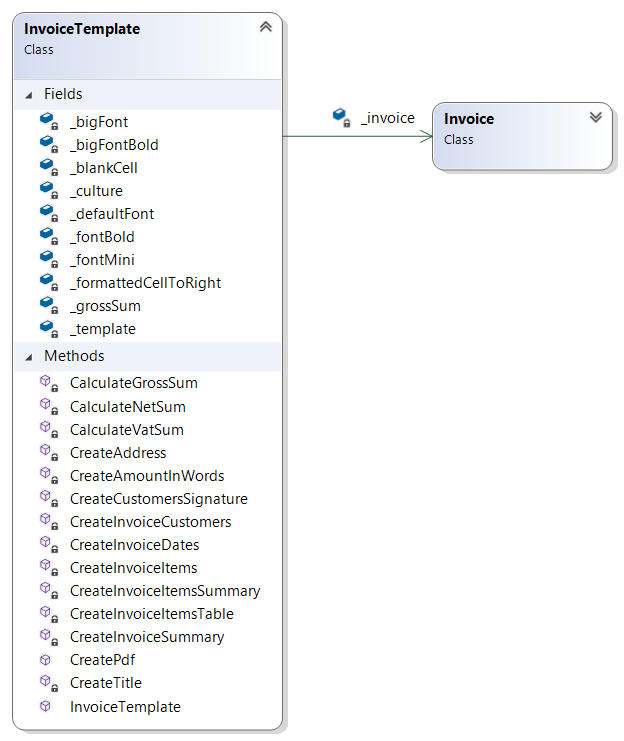
\includegraphics[width=0.6\linewidth]{Rysunki/InvoiceTemplate.png}
  \caption{Diagram klasy szablonu faktury}
  \label{fig:InvoiceTemplateDiagram}
\end{figure}

Główna metoda \textbf{CreatePdf} łączy wszystkie metody i generuje cały plik PDF.

\begin{lstlisting}[language={[Sharp]C},label=list:createPDF,caption=Metoda CreatePDF, basicstyle=\footnotesize\ttfamily]
public string CreatePdf(Utility.InvoiceTemplateStruct template)
{
    Document document = new Document(PageSize.A4, 50, 50, 70, 10);
    PdfWriter.GetInstance(document, new FileStream(file, FileMode.Create));

    document.Open();

    //create invoice title
    document.Add(_template.InvoiceType == Utility.InvoiceTypeTemplateEnum.Original
        ? CreateTitle("Oryginał", invoiceTitle)
        : CreateTitle("Kopia", invoiceTitle));


    document.Add(newLine);

    //create invoice date, invoice number and city
    document.Add(CreateInvoiceDates());

    document.Add(newLine);

    //create seller and contractor information
    document.Add(CreateInvoiceCustomers());

    document.Add(newLine);

    //create invoice items
    document.Add(CreateInvoiceItemsTable());

    document.Add(CreateInvoiceItems(_invoice.InvoiceItems.ToList()));

    document.Add(CreateInvoiceItemsSummary());

    document.Add(newLine);

    document.Add(CreateInvoiceSummary());

    for (int i = 0; i < 8; i++)
    {
        document.Add(newLine);
    }

    document.Add(CreateCustomersSignature());

    document.Close();

    return file;
}
\end{lstlisting}

Szablon generuje plik PDF na podstawie tworzenia tabel, które potem wypełniamy komórkami z danymi. Wszystkie metody w szablonie zwracają utworzoną tabelę, która dodawana jest do dokumentu za pomocą polecenia \textit{document.Add()}. W listingu \ref{list:createPDF} zostało pokazane złożenie wszystkich metod, które po kolei generują cały plik: 

\begin{enumerate}
    \item \textbf{CreateTitle} - utworzenie tytułu faktury (Faktura VAT, Faktura PRO FORMA lub korekta do faktury VAT) oraz dodanie czy faktura jest oryginałem czy kopią
    \item \textbf{CreateInvoiceDates} - utworzenie tabeli zawierającej daty sprzedaży i wystawienia faktury, miejsce wystawienia oraz numer faktury
    \item \textbf{CreateInvoiceCustomers} - dodanie do faktury danych sprzedawcy oraz nabywcy
    \item \textbf{CreateInvoiceItemsTable} - utworzenie tabeli dla pozycji z faktury
    \item \textbf{CreateInvoiceItems} - wypełnienie tabeli wszystkimi pozycjami znajdującymi się na fakturze
    \item \textbf{CreateInvoiceItemsSummary} - utworzenie podsumowania wszystkich pozycji (wyliczona suma netto, brutto oraz VAT)
    \item \textbf{CreateInvoiceSummary} - wygenerowanie podsumowania dla faktury (suma brutto liczbą oraz słownie, forma płatności, czy zapłacono, termin płatności, numer konta bankowego sprzedawcy oraz uwagi do faktury)
    \item \textbf{CreateCustomersSignature} - utworzenie miejsca na podpisy osób odpowiedzialnych za odbiór oraz wystawienie faktury
\end{enumerate}

Metody wyglądają podobnie. Tabele, które zwracają funkcje, różnią się jedynie układem oraz danymi. Przykładowa metoda:

\begin{lstlisting}[language={[Sharp]C},label=list:createTitle,caption=Metoda CreateTitle, basicstyle=\footnotesize\ttfamily]
private IElement CreateTitle(string invoiceType, string invoiceTitle)
{
    PdfPTable table = new PdfPTable(1);

    int[] colWidth = { 100 };
    table.SetWidths(colWidth);
    table.WidthPercentage = 100;

    PdfPCell invoiceTitleCell = new PdfPCell(new Phrase(invoiceTitle, _bigFontBold))
    {
        VerticalAlignment = Element.ALIGN_MIDDLE,
        HorizontalAlignment = Element.ALIGN_CENTER,
        Padding = 2,
        Border = 0
    };
    table.AddCell(invoiceTitleCell);
    PdfPCell invoiceTypeCell = new PdfPCell(new Phrase(invoiceType, _bigFont))
    {
        VerticalAlignment = Element.ALIGN_MIDDLE,
        HorizontalAlignment = Element.ALIGN_CENTER,
        Padding = 2,
        Border = 0
    };
    table.AddCell(invoiceTypeCell);

    return table;
}
\end{lstlisting}

W listingu \ref{list:createTitle} tworzona jest tabela z jedną kolumną o szerokości 100. Następnie są dodane do niej dwie komórki, które są wycentrowane w pionie i poziomie. Po każdym utworzeniu są dodawane do tabeli. Na koniec funkcja zwraca utworzoną tabelę, która dodawana jest do dokumentu.

\section{Projekt bazy danych}

Rysunek \ref{fig:erdDiagram} przedstawia diagram ERD bazy danych wraz z zależnościami między encjami. Kolejny diagram \ref{fig:erdDiagramForeign} został uzupełniony o klucze obce. Została pokazana także relacja między encjami oraz kluczami. Ostatni rysunek \ref{fig:erdDiagramAttr} został uzupełniony pozostałymi atrybutami encji.

\begin{figure}[ht!]
  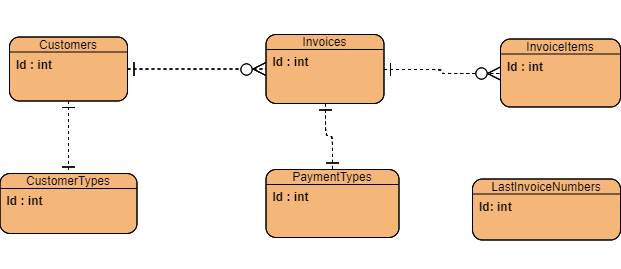
\includegraphics[width=\linewidth]{Rysunki/ERD.png}
  \caption{Diagram ERD w notacji Martina}
  \label{fig:erdDiagram}
\end{figure}

\begin{figure}[ht!]
  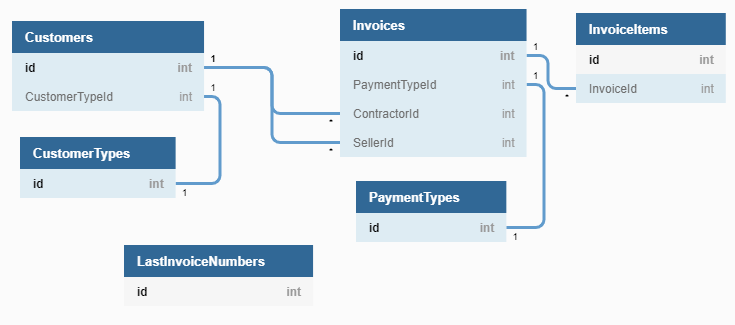
\includegraphics[width=\linewidth]{Rysunki/ERD-relacje.png}
  \caption{Diagram ERD uzupełniony o klucze obce}
  \label{fig:erdDiagramForeign}
\end{figure}

Opcjonalność encji:

\begin{itemize}
    \item Każda faktura (Invoices) \textbf{musi} posiadać jednego sprzedawcę i jednego kontrahenta (Customers)
    \item Każda faktura \textbf{może} posiadać produkty/elementy (InvoicesItems)
    \item Każdy element/produkt (InvoiceItems) \textbf{musi} znajdować się na fakturze (Invoices)
    \item Każdy klient (Customers) \textbf{musi} mieć zdefiniowany typ
    (CustomerTypes)
    \item Każda faktura \textbf{musi} mieć zdefiniowany typ płatności (PaymentTypes)
\end{itemize}

\begin{figure}[ht!]
  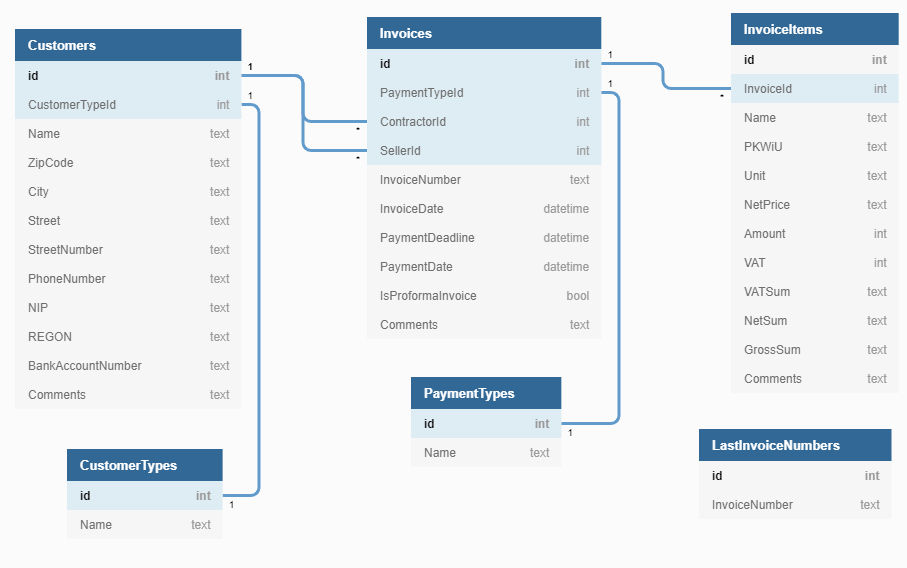
\includegraphics[width=\linewidth]{Rysunki/ERDAttr.png}
  \caption{Diagram ERD ze wszystkimi atrybutami encji}
  \label{fig:erdDiagramAttr}
\end{figure}

W tabelach \ref{tab:CustomerAttr}, \ref{tab:InvoicesAttr} i \ref{tab:InvoiceItemsAttr} zostały przedstawione wszystkie atrybuty jakie posiadają kolejno encje Customers, Invoices oraz InvoiceItems. Każdy atrybut posiada swój typ oraz krótki opis.

\begin{table}[ht!]
\centering
\resizebox{\textwidth}{!}{%
\begin{tabular}{|l|l|l|}
\hline
\textbf{Atrybut}  & \textbf{Typ}                                                       & \textbf{Opis}                                                                                                                             \\ \hline
Id                & \begin{tabular}[c]{@{}l@{}}INTEGER, \\ auto increment\end{tabular} & Klucz główny, unikalny, identyfikacja klienta                                                                                             \\ \hline
CustomerTypeId    & INTEGER                                                            & Klucz obcy, relacja z encją CustomerTypes                                                                                                 \\ \hline
Name              & TEXT                                                               & Nazwa firmy/klienta,                                                                                                                      \\ \hline
ZipCode           & TEXT                                                               & \begin{tabular}[c]{@{}l@{}}Kod pocztowy miasta, w którym znajduje się firma/\\ mieszka klient\end{tabular}                                \\ \hline
City              & TEXT                                                               & \begin{tabular}[c]{@{}l@{}}Nazwa miasta, w którym znajduje się firma/\\ mieszka klient\end{tabular}                                       \\ \hline
Street            & TEXT                                                               & \begin{tabular}[c]{@{}l@{}}Nazwa ulicy, na której znajduje się firma/\\ mieszka klient\end{tabular}                                       \\ \hline
StreetNumber      & TEXT                                                               & Numer budynku oraz numer lokalu                                                                                                           \\ \hline
PhoneNumber       & TEXT                                                               & Numer telefonu do firmy/klienta                                                                                                           \\ \hline
NIP               & TEXT                                                               & \begin{tabular}[c]{@{}l@{}}Numer identyfikacji podatkowej, \\ w formacie \#\#\#-\#\#\#-\#\#-\#\#\end{tabular}                             \\ \hline
REGON             & TEXT                                                               & \begin{tabular}[c]{@{}l@{}}numer identyfikacyjny REGON, \\ Rejestr Gospodarki Narodowej, \\ w formacie \#\#\#-\#\#-\#\#-\#\#\end{tabular} \\ \hline
BankAccountNumber & TEXT                                                               & Numer rachunku bankowego (26 cyfr)                                                                                                        \\ \hline
Comments          & TEXT                                                               & Uwagi do firmy/klienta                                                                                                                    \\ \hline
\end{tabular}%
}
\caption{Atrybuty encji Customers}
\label{tab:CustomerAttr}
\end{table}

\begin{table}[ht!]
\centering
\resizebox{\textwidth}{!}{%
\begin{tabular}{|l|l|l|}
\hline
\textbf{Atrybut}  & \textbf{Typ}                                                      & \textbf{Opis}                                                                                                                        \\ \hline
Id                & \begin{tabular}[c]{@{}l@{}}INTEGER,\\ auto increment\end{tabular} & \begin{tabular}[c]{@{}l@{}}Klucz główny, unikalny, \\ identyfikacja faktury\end{tabular}                                             \\ \hline
ContractorId      & INTEGER                                                           & Klucz obcy encji Customers                                                                                                           \\ \hline
SellerId          & INTEGER                                                           & Klucz obcy encji Customers                                                                                                           \\ \hline
PaymentTypeId     & INTEGER                                                           & Klucz obcy encji PaymentTypes                                                                                                        \\ \hline
InvoiceNumber     & TEXT, unique                                                      & \begin{tabular}[c]{@{}l@{}}Numer porządkowy faktury, jest unikalny, \\ format (kolejne liczby całkowite)/(aktualny rok)\end{tabular} \\ \hline
InvoiceDate       & TEXT                                                              & Data wystawienia faktury                                                                                                             \\ \hline
PaymentDeadline   & TEXT                                                              & Termin płatności za fakturę                                                                                                          \\ \hline
PaymentDate       & TEXT                                                              & Data płatności za fakturę                                                                                                            \\ \hline
IsProformaInvoice & INTEGER                                                           & \begin{tabular}[c]{@{}l@{}}Wartość binarna określająca czy faktura \\ jest fakturą pro forma, czy fakturą VAT\end{tabular}           \\ \hline
Comments          & TEXT                                                              & Uwagi do faktury                                                                                                                     \\ \hline
\end{tabular}%
}
\caption{Atrybuty encji Invoices}
\label{tab:InvoicesAttr}
\end{table}


\begin{table}[ht!]
\centering
\resizebox{0.8\textwidth}{!}{%
\begin{tabular}{|l|l|l|}
\hline
\textbf{Atrybut} & \textbf{Typ}                                                      & \textbf{Opis}                                                                                    \\ \hline
Id               & \begin{tabular}[c]{@{}l@{}}INTEGER,\\ auto increment\end{tabular} & \begin{tabular}[c]{@{}l@{}}Klucz główny, unikalny,\\ identyfikacja pozycji faktury\end{tabular}  \\ \hline
InvoiceId        & INTEGER                                                           & Klucz obcy encji Invoices                                                                        \\ \hline
Name             & TEXT                                                              & Nazwa pozycji                                                                                    \\ \hline
PKWiU            & TEXT                                                              & Polska Klasyfikacja Wyrobów i Usług                                                              \\ \hline
Unit             & TEXT                                                              & \begin{tabular}[c]{@{}l@{}}jednostka w jakiej jest zapisywana\\ pozycja na fakturze\end{tabular} \\ \hline
NetPrice         & TEXT                                                              & Cena netto pozycji                                                                               \\ \hline
Amount           & INTEGER                                                           & Ilość w jakiej kupujemy pozycję                                                                  \\ \hline
VAT              & INTEGER                                                           & Podatek VAT, podawany w procentach                                                               \\ \hline
NetSum           & TEXT                                                              & Suma netto pozycji                                                                               \\ \hline
GrossSum         & TEXT                                                              & Suma brutto pozycji                                                                              \\ \hline
VATSum           & TEXT                                                              & Różnica sumy brutto i netto                                                                      \\ \hline
Comments         & TEXT                                                              & Uwagi do pozycji                                                                                 \\ \hline
\end{tabular}%
}
\caption{Atrybuty encji InvoiceItems}
\label{tab:InvoiceItemsAttr}
\end{table}

W tabeli \ref{tab:entityRelations} przedstawiono relacje pomiędzy encjami. Encja Customers oraz Invoices połączone są relacją jeden do wielu, ponieważ każda faktura (Invoices) może posiadać jednego sprzedawcę i kontrahenta (Customers), a kontrahent oraz sprzedawca może znajdować się na wielu fakturach. Encja Invoices i InvoiceItems również jest połączona w relacji jeden do wielu. Każda faktura może mieć wiele produktów (InvoiceItems). Encje Customers i Invoices są w relacji 1:1 kolejno z encjami CustomerTypes (definiującej typ klienta - Sprzedawca oraz Kontrahent) oraz PaymentTypes (definiującej typ płatności za fakturę).

\begin{table}[ht!]
\centering
\resizebox{0.7\textwidth}{!}{
\begin{tabular}{|l|c|l|}
\hline
\textbf{Encja} & \multicolumn{1}{l|}{\textbf{Relacja}} & \textbf{Encja} \\ \hline
Customers      & 1:N                                   & Invoices       \\ \hline
Invoices       & 1:N                                   & InvoiceItems   \\ \hline
Customers      & 1:1                                   & CustomerTypes  \\ \hline
Invoices       & 1:1                                   & PaymentTypes   \\ \hline
\end{tabular}
}
\caption{Relacje między encjami}
\label{tab:entityRelations}
\end{table}

\section{Dobór technologii wytwarzania oprogramowania}
\subsection{Visual Studio 2019}
Najnowsze środowisko programistyczne \cite{VisualStudio} wydane przez firmę Microsoft w 2019 roku. Używane jest do tworzenia aplikacji konsolowych oraz oprogramowania z graficznym interfejsem użytkownika (np. Windows Forms, WPF czy aplikacji internetowych).

\subsection{C\#}
C\# \cite{CSharp} jest wysokopoziomowym, obiektowo zorientowanym \cite{CSharpBook} (rozdziały piąty, szósty oraz siódmy), językiem programowania. Programy napisane w tym języku są kompilowane do języka CIL (Common Intermediate Language), jest to kod pośredni wykonywany w środowiskach takich jak .NET Framework lub .NET Core. System operacyjny nie byłby w stanie uruchomić skompilowanego programu bez któregoś tych środowisk. Język C\# jest odpowiedzią Microsoftu na Javę. Był stworzony do pisania aplikacji na platformę Windows, teraz można również tworzyć w nim aplikację na platformy Linux, macOS. Aplikacje w języku C\# pisze się bardzo szybko o czym możemy przeczytać w książce \cite{CSharpBook} od strony 44. 

\subsection{.NET Core 3.0}
.NET Core 3.0 \cite{NetCore} to najnowszy framwework, którego premiera odbyła się 23 września 2019 roku. Oprogramowanie pozwala na tworzenie aplikacji dla platform Windows, Linux oraz macOS. Microsoft umożliwił tworzenie aplikacji WPF (Windows Presentation Foundation) w frameworku .NET Core od wersji 3.0. 

\subsection{WPF}
WPF, a dokładniej Windows Presentation Foundation \cite{WPF}, jest to silnik graficzny umożliwiający tworzenie aplikacji desktopowych. Interfejs programowania aplikacji opiera się na języku XML, a dokładniej na jego implementacji, która nazywa się XAML. Najważniejsze funkcje Windows Presentation Foundation zostały opisane w książce A. Nathana \cite{WPFBook} (na stronach 23-24 oraz 27-29). 

\subsection{Microsfot.EntityFrameworkCore}
Entity Framework Core \cite{EFCore} jest to open source'owa platforma programistyczna ułatwiająca korzystanie z baz danych oraz operacji CRUD. Entity Framework umożliwia programistom pracę z bazą danych przy użyciu obiektów .NET, eliminując tym samym potrzebę korzystania z zapytań SQL. Bardzo pomocna okazała się książka P. Anbazhagan \cite{EFCoreBook}, w której krok po kroku opisana jest cała konfiguracja Entity Framework Core do projektu. Pozycja bibliograficzna skupia się na zastosowaniu EF Core w ASP .NET, jednak w Windows Presentation Foundation wygląda to bardzo pdoobnie.

\subsection{Microsoft.Extensions.DependencyInjection}
Dependency Injection jest to wzorzec projektowy pozwalający na usunięcie zależności pomiędzy komponentami, na rzecz architektury \textbf{plug-in}. Polega na przekazaniu gotowych instacji obiektów, obiektom, które z nich korzystają (np. jako parametry konstruktora).

\subsection{SQLite}
W projekcie została użyta baza danych SQLite, z kilku prostych powodów \cite{UsingSQLite}:
\begin{itemize}
    \item Baza nie potrzebuje serwera do poprawnego działania (użytkownik nie musi instalować innego pośredniczącego oprogramowania, żeby uruchomić aplikację)
    \item Baza danych zawarta jest w jednym pliku (łatwe przeglądanie bazy danych)
    \item Umożliwia dostęp z kilku różnych procesów oraz wątków
    \item Zapewnia większość podstawowych zapytań SQL
\end{itemize}

\subsection{Github}
W projekcie zostało użyte narzędzie Github \cite{GithubBook} w celu kontrolowania wersji aplikacji. Narzędzie było bardzo przydatne przy wprowadzaniu nowych funkcjonalności. W przypadku jakichkolwiek błędów, zawsze można było wrócić do poprzedniej wersji aplikacji.

\subsection{Biblioteki}

\subsubsection{MaterialDesignInXamlToolkit}
MaterialDesignInXamlToolkit \cite{MaterialDesignXAML} jest open source'ową biblioteką, która zmienia domyślny wygląd kontrolek WPF. Material Design to system projektowy stworzony przez Google, który łączy zasady dobrego designu wraz z innowacyjnymi możliwościami technologicznymi.

\subsubsection{LiczbyNaSlowaNetCore}
LiczbyNaSlowaNetCore \cite{LiczbyNaSlowa} jest to open source'owa biblioteka do zamiany liczb na słowa. Konwertuje liczby zarówno całkowite jak i zmiennoprzecinkowe.

\subsubsection{iTextSharp}
iTextSharp \cite{itext} jest open source'owym narzędziem do tworzenia plików PDF. W projekcie zostało użyte w celu generowania faktur.

\section{Proponowane wymagania sprzętowe i programowe}